\documentclass[a4paper,12pt,twoside,openright,titlepage]{book}

%Additional packages
\usepackage[utf8]{inputenc}
\usepackage[T1]{fontenc}
\usepackage[dutch,english]{babel}
\usepackage{imakeidx}
\usepackage{syntonly}
\usepackage[official]{eurosym}
%\usepackage[graphicx]
\usepackage{graphicx}
\graphicspath{ {./images/} }
\usepackage{float}
\usepackage{xurl}
\usepackage{hyperref}
\hypersetup{colorlinks=true, linkcolor=blue, citecolor=blue, filecolor=blue, urlcolor=blue, pdftitle=, pdfauthor=, pdfsubject=, pdfkeywords=}
\usepackage{tabularx}
\usepackage[table]{xcolor} % Table colors
\usepackage{scrextend}
\addtokomafont{labelinglabel}{\sffamily}
\usepackage{listings}
\usepackage{adjustbox}
\usepackage{color}
\usepackage{csquotes}

% Define colors
\definecolor{ashgrey}{rgb}{0.7, 0.75, 0.71}

% Listing style
\lstset{
  backgroundcolor=\color{ashgrey}, % choose the background color; you must add \usepackage{color} or \usepackage{xcolor}; should come as last argument
  basicstyle=\footnotesize,        % the size of the fonts that are used for the code
  breakatwhitespace=true,          % sets if automatic breaks should only happen at whitespace
  breaklines=true,                 % sets automatic line breaking
  extendedchars=true,              % lets you use non-ASCII characters; for 8-bits encodings only, does not work with UTF-8
  frame=single,	                   % adds a frame around the code
  rulecolor=\color{black},         % if not set, the frame-color may be changed on line-breaks within not-black text (e.g. comments (green here))
  keepspaces=true,                 % keeps spaces in text, useful for keeping indentation of code (possibly needs columns=flexible)
  columns=fullflexible,		   % make copy and paste possible
  showstringspaces=false,          % if true show spaces in strings adding particular underscores
  showspaces=false,                % if true show spaces everywhere adding particular underscores; it does not override 'showstringspaces'
}

% Uncomment for production
% \syntaxonly

% Style
\pagestyle{headings}

% Turn on indexing
\makeindex[intoc]

% Define document
\author{D. Leeuw}
\title{Elektriciteit}
\date{\today\\v.0.8.0}

\begin{document}
\selectlanguage{dutch}

\maketitle

\copyright\ 2023 Dennis Leeuw\\

\begin{figure}

\includegraphics[width=0.3\textwidth]{CC-BY-SA-NC.png}
\end{figure}

\bigskip

Dit werk is uitgegeven onder de Creative Commons BY-NC-SA Licentie en laat anderen toe het werk te kopi\"eren, distribueren, vertonen, op te voeren, en om afgeleid materiaal te maken, zolang de auteurs en uitgever worden vermeld als maker van het werk, het werk niet commercieel gebruikt wordt en afgeleide werken onder identieke voorwaarden worden verspreid.


%%%%%%%%%%%%%%%%%%%
%%% Introductie %%%
%%%%%%%%%%%%%%%%%%%

\frontmatter
\chapter{Over dit Document}
\input{src/OverDitDocument}
\input{src/DocChanges}

%%%%%%%%%%%%%%%%%
%%% De inhoud %%%
%%%%%%%%%%%%%%%%%
\tableofcontents

\mainmatter
\chapter{Inleiding}
Dit document behandeld de elektronica die nodig is computersystemen tot op component niveau te kunnen begrijpen. Het beschrijft de verschillende componenten in de elektronica die gebruikt worden om een computer te maken en hoe deze samen gebruikt worden om de 1 en 0 in een computer te maken.


\chapter{Stroom}
Elektriciteit is het verplaatsen van geladen deeltjes door een materiaal. In de meeste gevallen zijn het elektronen die door het materiaal bewegen.

De bouwstenen van alle materialen zijn atomen. Atomen zijn de kleinste deeltjes die nog de eigenschap van een materiaal bevatten. Het kan nog kleiner, maar dan veranderen ook de eigenschappen. Een atoom is opgebouwd uit protonen, elektronen en mogelijk ook neutronen. Zoals de naam al aangeeft zijn neutronen neutraal, dat wil zeggen dat ze geen lading hebben. Protonen en elektronen hebben wel een lading. Protonen zijn positief geladen deeltjes en elektronen negatief geladen deeltjes. Net als bij magneten de noord-pool de zuid-pool aantrekt, trekken de positieve deeltjes de negatieve deeltjes aan.

Stoffen opgebouwd uit atomen lijken voor ons soms heel massief en hard, maar in werkelijkheid bestaan ze uit vrij veel lege ruimte. Een atoom bestaat uit een atoomkern met daar omheen elektronen. Net zoals de planeten om de zon draaien. De atoomkern bestaat uit protonen en neutronen en is behoorlijk massief, maar de elektronen draaien op relatief veel afstand van de kern. Het zijn deze elektronen die kunnen bewegen en van atoom naar atoom kunnen stromen.

Leggen we nu een reeks koperatomen op een rij dan hebben we een koperdraad. Als die 1 atoom dik zou zijn dan wordt het allemaal wat heel erg klein, maar als we de dikte ook van meerdere atomen maken dan begint het al meer op stroomdraad te lijken. Knippen we deze draad in 2 gelijke stukken en verbinden we de ene kant van elke draad met een lamp en de andere met de + of de - zijde van een batterij dan kunnen de elektronen van de - kant van de batterij door de koperdraad naar de lamp bewegen en van de lamp door de andere koperdraad weer terug naar de + kant van de batterij. We kunnen dan dus elektronen doorgeven. Het doorgeven van elektronen gebeurt in een stroomkring.

Elektronen zijn negatief geladen deeltjes en die stromen van de negatieve (-) kant naar de positieve (+) kant. De wetenschappers wisten toen ze elektrotechniek ontdekten niets van elektronen en hebben toen bepaald dat stroom de beweging van positieve deeltjes is van + naar -. Het maakt voor de werking van de elektrotechniek niet uit of je fictieve positieve deeltjes hebt die van de plus naar de min lopen of werkelijke negatieve deeltjes die van de min naar de plus lopen. Het effect is hetzelfde, er wordt lading verplaatst.

De stroom heeft als symbool de I\index{I} en wordt uitgedrukt in Amp\`ere\index{Amp\`ere}, afgekort de A\index{A}. We spreken van een stroom van bijvoorbeeld 5 A. \[ I = 5 A \].


\section{Opdracht}
Vul een plastic buis met pingpong ballen. Druk er nog een extra bal in en neem waar dat er 
\begin{enumerate}
\item Kracht nodig is om de pingpong bal erin te drukken
\item Bij elke extra bal die er bij de ingang in gaat er een bal bij de uitgang uitkomt
\end{enumerate}

De kracht die je moet gebruiken om er een pingpongbal in te drukken is vergelijkbaar met de spanning die nodig is om elektronen te laten bewegen.

Het verlies van pingpong ballen aan het uiteinde is natuurlijk zonde. Als je de pingpongbal weer opraapt en er aan het begin weer instopt, dan scheelt dat een hoop pingpongballen. Zo werkt het in de natuur ook. Elektronen lopen rond, je hebt dus een stroomkring nodig voor elektriciteit.


\chapter{Spanning}
Uit de wandcontactdoos komt 230 Vac. Dat is de spanning\index{Spanning}, of het potentiaalverschil\index{Potentiaalverschil}. AA penlite batterijen hebben een spanning van 1,5 Vdc.

Als we de vergelijking maken met water, dan is de spanning vergelijkbaar met de druk. Als we een emmer met water op een trap zetten en in die emmer met water zit aan de onderkant een kraantje, dan staat er een bepaalde druk op de uitgang van de kraan. Als we de kraan dicht laten gebeurd er niets en toch is er die druk. Draaien we de kraan open dan stroomt er water. Zolang de emmer niet leeg is blijft er druk staan op het water. Zo werkt een batterij ook. Zolang als er spanning in de batterij zit kan er stroom lopen. Is de batterij leeg, dan is er geen spanning meer en ook geen stroom.

Het symbool voor de spanning is de U\index{U} en de eenheid is de V\index{V}, ofwel de Volt\index{Volt}. Voor de AA penlite batterij geldt dus: \[ U = 1,5 V \].

Achter de V kan een toevoeging komen, namelijk ac of dc. Deze termen zijn afkortingen en staan voor Alternating Current\index{Alternating Current}\index{AC} en Direct Current\index{Direct Current}\index{DC}. Of wel wissel stroom en gelijk stroom. AC en DC zijn Engelse termen. In het Nederlands spreken we wisselspanning of gelijkspanning terwijl we wel de afkortingen ac en dc gebruiken.

Bij een gelijkspanning\index{Gelijkspanning} blijft de 'druk' constant. Een batterij heeft een gelijkspanning. De batterij zal, als hij niet leeg is, continue een spanning hebben van 1,5 Volt.

Een wisselspanning\index{Wisselspanning} heeft, zoals de naam al aangeeft, een wisselende spanning. De spanning beweegt van het maximum, via de 0 naar een minimum en weer terug via een sinus-vorm, zie \ref{fig:sinus}.

\begin{figure}[h]
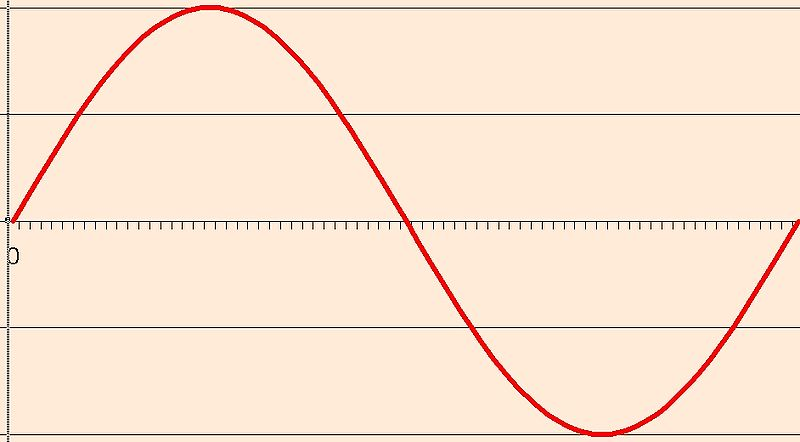
\includegraphics[width=5cm]{800px-Sinus}
\centering
\caption{Tekening door Philip Bosma (\url{https://commons.wikimedia.org/wiki/File:Sinus.jpg})}
\label{fig:sinus}
\end{figure}

De spanning uit het stopcontact maakt deze beweging 50 keer per seconde en heeft dus een frequentie van 50 Hz.


\section{Opdracht}
Neem een batterij en een multimeter. Meet met de multimeter de spanning van de batterij.


\chapter{Weerstand}
Als we de + en de - van een batterij met elkaar verbinden dat maken we een kortsluiting. Bij een kortsluiting gaat er heel veel stroom lopen, zoveel zelfs dat het plastic om de geleider in brand zou kunnen vliegen. Om te voorkomen dat dat gebeurd moeten we de stroom beperken. Dit doen we door de weerstand\index{Weerstand} te verhogen. De weerstand vermindert de stroom en daardoor ontstaat er geen brand.

Er zijn verschillende manieren om de weerstand te verhogen. We kunnen gebruik maken van een apparaat dat de stroom gebruikt om te werken (bijvoorbeeld een lamp die brandt), maar we kunnen ook een speciaal stukje elektronica gebruiken, genaamd een weerstand\index{Weerstand}\index{Resistor} die als enige functie heeft de weerstand in een circuit te verhogen zodat de stroom beperkt wordt.

In de elektronica wordt een weerstand weergegeven met het symbool dat je ziet weergegeven in \ref{symbool:weerstand}

\begin{figure}[h]
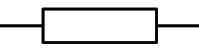
\includegraphics[width=5cm]{weerstand}
\centering
\caption{Symbool van een weerstand}
\label{symbool:weerstand}
\end{figure}


\section{De wet van Ohm}
De elektrische stroom loopt door de stroom draad, maar eigenlijk zijn het elektronen die door de draad bewegen. Het bewegen door de draad kost moeite. In de draad zit een bepaalde weerstand\index{Weerstand} die door de elektronen overwonnen moet worden. Door een potentiaal verschil (spanning) aan te leggen kunnen we de elektronen door de draad drukken. Er is dus een relatie tussen de spanning, de stroom en de weerstand van de kabel.

In 1826 toonde George Ohm\index{Ohm} deze relatie aan en vatte die in een formule die naar hem genoemd is: De wet van Ohm\index{Wet van Ohm}. De formule die daarbij hoort is \[ R = \frac{U}{I} \]

R is hierbij de weerstand die wordt uitgedrukt in aantallen ohm ($\Omega$). Als er bij een spanning van 1,5 V een stroom door de draad loopt van 2 A, dan geldt voor de weerstand van die draad: \[ R = \frac{1,5}{2} = 0,75 \Omega \]

De formule wordt vaker geschreven als: \[ U = I*R \]



\chapter{Arbeid en vermogen}
Bij het gebruik van energie gaat het uiteindelijk om het verrichten van arbeid. Als we een electrische auto laten rijden wordt er arbeid verricht, zo ook bij het branden van een lamp en bij het zetten van koffie met een koffiezetapparaat. Electrische energie wordt omgezet in een energie vorm die we op dat moment nodig hebben. Bij een lamp wordt electrische energie omgezet in licht, bij auto in beweging en bij een koffiezetapparaat in warmte om het water aan de kook te brengen.

Om electriciteit deze arbeid te laten verrichten hebben we een stroomkring nodig. De energie gaat van de energie opwekker, naar de verbruiker en weer terug naar de opwekker.

Het is te vergelijken met een schoepenrad in een rivier. De zon verwarmt de zee en verdampt zo water. Water drijft in wolken naar de kust. Boven het land valt het water naar beneden in de vorm van regen, sneeuw of hagel. Uiteindelijk komt het water in een rivier terecht en door de zwaartekracht wordt het stroomafwaarts vervoert naar de zee. De kringloop kan opnieuw beginnen. Als we gebruik willen maken van de energie van de rivier dan kunnen we een schoepenrad plaatsen en via een as bijvoorbeeld een molensteen aandrijfen om graan te malen. Er blijft dezelfde hoeveelheid water door de rivier stromen, en toch hebben we bewegingsenergie van de rivier gebruikt om graan te malen.

In de electrotechniek gebeurt hetzelfde. Het water uit de rivier is te vergelijken met de stroom die loopt door een stroomkring. Een batterij is een stroombron, dus die levert stroom, via een koperdraad gaat dit naar een lamp, die geeft licht, en van de lamp gaat de stroom via een koperdraad terug naar de batterij. Bij de rivier is het de zwaartekracht die ervoor zorgt dat het water stroomt en bij de batterij is het de spanning die ervoor zorgt dat de stroom stroomt.

De hoeveelheid arbeid die verricht wordt door de lamp die electriciteit omzet in licht is het vermogen dat gebruikt wordt en vermogen wordt uitgedrukt in Watt. In de winkel staat dan ook altijd op een lamp hoeveel Watt deze is.

We kunnen het vermogen van de rivier op twee manieren be\"invloeden. We kunnen er meer water doorsturen, of we kunnen een stijlere rivier nemen zodat het water sneller stroomt. Ditzelfde geldt voor electriciteit, we kunnen meer stroom laten vloeien door de spanning te verhogen. Hieruit blijkt dat spanning, stroom en vermogen van elkaar afhankelijk zijn. Die afhankelijkheid kunnen we weergeven in een formule:

\[ P = U*I \]

P = Vermogen
U = Spanning
I = Stroom

Als ik de spanning verdubbel, bij een gelijk blijvende stroom, verdubbelt dus het vermogen. Zo geldt ook dat als ik het vermogen constant hou en de spanning verdubbel, de stroom dus moet halveren.

Een andere manier om meer stroom te laten lopen is door de weerstand te verlagen. De weerstand is te vergelijken met de obstakels in een rivier. Liggen er heel veel stenen in de rivier waar het water op botst dan zal de stroomsnelheid afnemen. Nemen we de stenen weg dan zal de rivier sneller stromen. In de electronica geldt hetzelfde. In onze eenvoudig stroomkring met een batterij, twee stukken koperdraad en een lamp kunnen we niet zo veel doen om de weerstand te verlagen, we kunnen hem echter wel eenvoudig verhogen. Door een weerstand op te nemen in het circuit kunnen we een extra \textquote{steen} in de stroomkring aanbrengen zodat er minder stroom loopt.

Dus door een weerstand toe te voegen loopt er bij gelijk blijvende spanning minder stroom. Hieruit mogen dus vaststellen dat er een relatie is tussen spanning, stroom en weerstand. En die is er ook, die relatie heet de wet van Ohm:

\[ U = I*R \]

U = Spanning
I = Stroom
R = Weerstand

Door de weerstand in het circuit loopt er minder stroom, de lamp kan dus minder arbeid verrichten en zal minder fel gaan branden. Het vermogen (verbruik van de lamp) neemt dus af. Als we willen weten wat het vermogen van de lamp is nadat we de weerstand hebben toegevoegd dan moeten we de twee voorgaande formules combineren:

\[ P = U^2/R \]

P = Vermogen
U = Spanning
R = Weerstand

Deze combinatie wordt gemaakt door substitutie. Substitutie is een moeilijk woord voor vervanging. In de formule P=U*I hebben we de I vervangen door de I uit U=I*R. Om te weten wat de I is uit U=I*R moeten we delen door hetzelfde "getal" aan beide kanten van het = teken. Dus als we I*R delen door R dan houden we I over. Nu moeten we ook delen door R aan de U kant, we houden dus U/R over:

U/R = I

Nu we weten wat I is kunnen we dat in de formule voor het vermogen stoppen:

\[ P = U*(U/R) = U^2/R \]

En we zien nu dat bij een gelijkblijvende spanning, het vermogen van de lamp direct afhankelijk is van de weerstand. Als we de weerstand 2x zo groot maken zal het vermogen 2x zo klein worden. Er is dus een omgekeerde afhankelijkheid tussen het vermogen en de weerstand.

Omdat we in de elektronica elektronen door materiaal duwen, wordt er arbeid\index{Arbeid} verricht en deze arbeid wordt voor een bepaalde tijd verricht. De P\index{P} heeft dan het vermogen en de eenheid die daar bij hoort is de Watt\index{Watt} (W\index{W}). Als we dit vermogen een uur lang gebruiken dan spreken we van een Wh\index{Wh} (Watt-uur). Bij 1000 Wh korten we dit af tot een kWh\index{kWh} ofwel een kilo-Watt-uur.



%%%%%%%%%%%%%%%%%%%%%
%%% Index and End %%%
%%%%%%%%%%%%%%%%%%%%%
\backmatter
\printindex
\end{document}

%%% Last line %%%
